\raggedbottom

\chapter{Game Development}
\label{cha:game_development}

This chapter addresses the technical details chosen to develop the mini-games. Before and during the creation of the mini-games, it is important to correctly detail the looks as well as the tools and technologies used to generate the best architecture.
Section \ref{designPriciples} will start by focusing on the design principles that were taken into account, followed by the technologies used, explaining each choice in the section \ref{methodology}. 
To create these many mini-games a good foundation is needed hence the reason for clear modelling of the software before hands-on work. Section \ref{arqOverview} will go through an overview for the proposed arquitecture that will be utilized in every game.

Finally, we will be able to see the each game's implementation on its own from sections \ref{arqHearts} to \ref{arqPuzzle}.

\newpage
\section{Design Principles and Accessibility Considerations}
\label{designPriciples}

Design is a huge aspect of games, specially the ones being developed in this project. In order to help children with Learning Disabilities, not only the games structure have to be well written but their visuals have to encourage children to learn and play the games.

This section aims to describe the game's structure design. We'll specify each aspect of the game regarding the following topics: \textbf{Colors}, \textbf{Dimensional Structure} (2D or 3D), and \textbf{Style}.

\subsection*{Color}
The colors have to be carefully chosen, not only for the game to be more exciting for the players, but also, in this specific case it has to be tailored specifically to children with learning disabilities.
For this, we maintain a \textbf{high contrast for clarity} across all games, meaning that all colors have a high contrast between the background and the objects. This is a highly important characteristic as it can help children with Visual Motor Deficit and Dyslexia.
At the same time, it is also very important to keep a \textbf{soft and calming palette} of colors creating a non-overstimulating environment. This can benefit children with \textbf{Dyslexia}, \textbf{Visual Motor Deficits}, and \textbf{Non-Verbal Learning Disabilities}, reducing visual stress and enhancing their ability to process visual information.

\subsection*{Dimensional Structure}
As previously seen, the games where all build using a 2D structure. While the developing of a game for children with learning disabilities in 3D is possible, it can never be compared to the decrease in complexity to a 2D environment. 2D games are generally of more \textbf{simple navigation and interaction}. They also keep the presentation of the games more straightforward removing the necessity for more details.

\subsection*{Style}
There are several types of styles such as: Realistic, Minimalistic, Retro/Pixel-Art, Cartoonish, etc.
It's important to note that the mini-games should follow only one style. A \textbf{consistent art style} lets the children to know what to expect, while too much change in the visuals might be too overwhelming for children with \textbf{Language Processing Disorder}, as consistency helps reduce cognitive load.

The chosen style was the \textbf{cartoonish}, which helps provide an enganing and friendly environment for children. Simple characters like animals, hearts, or flowers increase \textbf{emotional engagement} and create a playful environment.

Because it is \textbf{simple and clean}, this style also helps remove any visual clutter that can be distracting or confusing, making it easier to focus on the task at hand and generating an immediate understanging of each game.

With this in mind, it is important to know where to get images and assets for the development of the mini-games. Nowadays, most of the assets found online are protected and can't be used in public domain. Despite this, some assets for the games have been found online and certified that they can be used in a project context. For this purpose, we used the websites like \textbf{Icons8} (\url{www.icons8.com}) and \textbf{FreePik} (\url{www.freepik.com}).

All other assets are composed with the use of Artificial Intelligence (excluding some developed locally) with the help of Adobe's AI tools in Adobe Photoshop. All the backgrounds for the mini-games have been generated with AI, allowing for commercial use \cite{adobeGuidelines}.

% \newpage
\subsection*{Design Overview}
% TODO: detalhar a estrutura dos jogos

Before detailing each game, it is important to develop the flow for each one. The games can be rather different from one another, but to keep the same language between all of them we utilized the following flow. When the player opens a game he/she will be greated with a home page with all the necessary instructions to be aquanted with the current game. After this, each game will always have some kind of different levels or difficulties to choose from.
Because of this, the folowing wireframes were made, depicted in figures \ref{fig:home-wireframe} and \ref{fig:levels-wireframe}. After these screens the game shall begin.

\begin{figure}[H]
    \centering
    \begin{minipage}{0.45\textwidth}
      \centering
      
\includegraphics[width=\linewidth]{Chapters/figma/home-wireframe.png}
      \caption{Game Home Page Wireframe}
      \label{fig:home-wireframe}
    \end{minipage}
    \hfill
    \begin{minipage}{0.45\textwidth}
      \centering
      
\includegraphics[width=\linewidth]{Chapters/figma/levels-wireframe.png}
      \caption{Levels Page Wireframe}
      \label{fig:levels-wireframe}
    \end{minipage}
\end{figure}

% Color Choices
% Style and Visual Simplicity
% 2D Design
% Game-Specific Insights

\section{Methodology, Tools, and Techniques}
\label{methodology}
There are many ways to go about building a game, a lot of frameworks, tools, programming languages, etc. The first decision made was to use an existing game engine that already exists. A \textbf{game engine} is a tool that allows the creation of video games without the hassle of building everything from the ground up. This means that any types of assets such as textures, sounds, \gls{ui}, are already available to use and there is no need to create any type of mechanism to place something on the screen for instance, it abstracts most of the technical details making so that the developer is able to use it and create games in much less time. There are a few game engines that are free to use such as Unity \cite{unity}, Unreal Engine \cite{unrealengine}, Godot \cite{godot}, Game Maker \cite{gamemaker}, LibGDX \cite{libgdx}, among others.
It is important to understand what are the main characteristics of the games and to narrow the options based on that.
Here we're looking to build 2D mini-games that are not graphically demanding and that can easily be ported to PC, MacOS, Android, or iOS.

It was decided to use Unity due to its support of lots of features regarding 2D game development, the ability to build to almost any platform and also already having quite some experience with the tool.

Because the mini-games have impact on the users through user experience it is also an important step to choose the tool used to prototype every screen present in the game before any development. For that, we will be using Figma \cite{figma}, a free prototyping tool owned by Adobe that will allow for creating the best scenarios for each screen present in the project. There is also the possibility to ask for feedback from friends and family right before the development, ensuring that almost no time is spent changing layouts or user flows.

\section{Unity Components}
Unity uses the C\# programming language to manipulate the game structure but it can also be used with visual scripting. C\# is an \gls{oop} language so it's great for creating a good architecture using principles like polymorphism, encapsulation, inheritance, and abstraction.

Unity uses a script like system in which every asset that is present in the scene is called a \textbf{GameObject} and through these we can introduce C\# scripts that will then manipulate the logic in the game. Each script acts as a component of the GameObject and is required to extend the base class \textit{MonoBehaviour} from the Unity Engine's library \cite{unityDocMonoBehaviour}.

This class offers the support for multiple event functions \cite{unityDocEvent}, such as:

\begin{itemize}
    \item \textbf{Regular Update Events} - Update functions are frequently called in order to update each object state before rendering the next frame. The main function is the \textit{Update()} function, but there is also a \textit{FixedUpdate()} that updates in discrete time steps in a similar way to the frame rendering.

    \item \textbf{Initialization Events} - These events are called in the initialization of objects. The \textit{Start()} function is called right before the first frame update. There is also the \textit{Awake()} function that is called for each object when the scene is loaded. 
    
    \item \textbf{GUI events} - Graphical User Interface events are also available to handle user interactions. Some of these events are the \textit{OnMouseDown()}, \textit{OnMouseOver()}, and \textit{OnMouseExit()} events that help detecting mouse events.
    
    \item \textbf{Physics events} - Physics events are also available to detect collisions and triggers such as \textit{OnCollisionEnter()}, \textit{OnTriggerEnter()}, \textit{OnCollisionExit()}, and \textit{OnTriggerExit()}.
\end{itemize}

% \begin{itemize}
%     \item \textbf{Start()}: <explain here>
%     \item \textbf{Update()}: <explain here>
%     \item \textbf{FixedUpdate()}: <explain here>
%     \item \textbf{LateUpdate()}: <explain here>
%     \item \textbf{OnDisable()}: <explain here>
%     \item \textbf{OnEnable()}: <explain here>
% \end{itemize}

There are also objects that can exist independently of GameObject such as the \textbf{\textit{Scriptable Object}}. Classes that extend this base class are used to centralise data to facilitate access from scenes and assets within a project \cite{unityDocScriptableObj}.

% https://docs.unity3d.com/ScriptReference/MonoBehaviour.html
% https://docs.unity3d.com/ScriptReference/ScriptableObject.html


\newpage

\section{Architecture Overview}
\label{arqOverview}
Since C\# is an \gls{oop} language, we have the possibility to use all the principles found in this paradigm such as:

\begin{itemize}
    \item \textbf{Inheritence} - The ability to have an object that inherits it's base from a super component (eg the object Truck can inherit characteristics from Car).
    \item \textbf{Encapsulation} - The ability of hiding the internal state of an object from the consumer.
    \item \textbf{Polymorphism} - The ability to have operations with a given name, that perform the same operation in different ways.
    \item \textbf{Abstraction} - The ability of hiding complexities and implementations exposing simpler objects.
\end{itemize}

Using these simple principles, the output is easier to understand with less entropy in the creation as well as debugging of the project. It also helps reusing code that can be used multiple times.

The implementation will be contained in a package called \textbf{minigames}. Here we can expect a package for each mini-game (\textbf{hearts}, \textbf{maze}, \textbf{sounds}, \textbf{puzzle}, and \textbf{words}) but also another one for the game home scene that will also require some implementation. Lastly, there will be a package called \textbf{common} which will handle any type of operations that can be used for multiple games. An example could be a counter that can be used in multiple games and has the same implementation in all of them.

The implementation can be found in the following Azure Repository: \url{https://dev.azure.com/A45414/_git/Thesis%20Children%20Learing%20Disabilities}.

% TODO: Add leantween library

\newpage
Figure \ref{fig:packages} shows the package structure.

\begin{figure}[H]
    \centering
    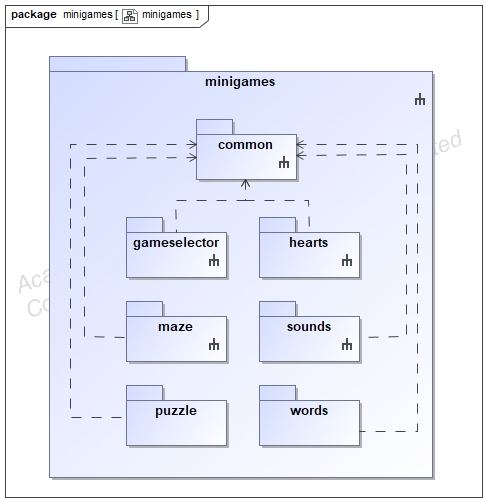
\includegraphics[scale=.5]{Chapters/arq/class__minigames__minigames.jpg}
    \caption{Overall Application Architecture}
    \label{fig:packages}
\end{figure}

The idea is to develop a common structure which will be used by the five mini-games making it easier to create each one with the same structure. 

It will consist of abstract handlers that contain a small chunk of implementation that applies for all games. This solution design aims at reducing entropy and ambiguity as much as possible, allowing for the developer to focus solely on each game development one by one.

The main components for this architecture are as follows:
\begin{itemize}
    \item \textbf{\textit{GameHandling}}.
    \item  \textbf{\textit{MenuHandling}}.
    \item \textbf{\textit{ScoreManager}}.
    \item \textbf{\textit{ScenesHandling}}.
\end{itemize}

% TODO Explain a MonoBehaviour

% The main components for this architecture will be responsible for handling the game logic and the the user menus (\textbf{\textit{GameHandling}} and \textbf{\textit{MenuHandling}}).

\newpage
\paragraph{\textit{GameHandling}} allows for a variety of operations, but it mainly allows the game to support basic funcionalities such as:

\vspace{-\topsep}  % Reduce space before itemize
\begin{itemize}
    \setlength{\itemsep}{8pt}  % Removes extra space between items
    \setlength{\parskip}{0pt}  % Removes space between paragraphs within items
    \item Start and finish game.
    \item Exit and restart game.
    \item Managing game state.
\end{itemize}
\vspace{-\topsep}  % Reduce space before itemize

Because we're using Unity where most of the scripts will be attached to GameObjects and not directly connected to these mechanisms, \textit{GameHandling} hosts two separate events capable of notifying components of Start and Finish game events.

It utilizes the Observer Design Pattern \cite{observer} which allows the definition of a subscription mechanism to notify multiple objects about these events on the game status.

\textbf{\textit{GameHandling}} is also responsible for loading the game and therefore has an unimplemented method `LoadDifficultyLevel' which after implementation is able to load any game. It's important to notice that each game may have it's definition of a difficulty level and for that reason this object allows for any time of level needed.\\

\paragraph{\textit{MenuHandling}} is responsible for user interaction with game menus such as `levels menu', `scores menu', and `pause menu'. It has two important methods `HidePanel' and `OpenPanel', able of opening and closing any menu with an expanding animation. On these methods, the developer should specify all the menus and interactions they should have. It contains several operations that are present in all the games such as:

\begin{itemize}
    \item Dealing with the choosing Levels Menu (`OpenLevelMenu', `HideLevelMenu', `GoBackToGameButton').
    \item Opening and closing the audio settings (`OpenAudioSettings', `CloseAudioSettings')
    \item Dealing with the end of a game (`ShowScoresFinish', `OpenGameFinishOptions')
    \item Reading instructions out loud (`ReadInstructionAloud', `StopInstructions', `PlayAudioSequentially')
\end{itemize}

It keeps a reference to the `GameHandling' (generic objects `T' and `V') and the `ScoreManager' (generic object `A' means the type of the score) of the game and if necessary performs changes.\\

\paragraph{\textit{ScoreManager}} is an abstract component that holds and saves the game scores. It is created once in the `GameHandling' object. It has several operations that allow for the setting and getting of the scores. Because scores can differ between mini-games, the score itself only has the constraint of being an object that implements the C\# Interface \textit{IComparable}, allowing multiple scores to be compared.

Because the `MenuHandling' and `ScoreManager' need to be accessed at any time from any Object, the Singleton pattern was considered \cite{singleton}. This is a design pattern present in object oriented programming languages and ensures that a class has only one instance, while providing a global access point to the instance.

\paragraph{\textit{ScenesHandling}} is a static data object that stores all the names of each mini-game as constants, removing ambiguity while navigating between scenes from anywhere.

Figure \ref{fig:handlers} represents the complete architecture of this mechanism in \gls{uml}.

\begin{figure}[H]
    \centering
    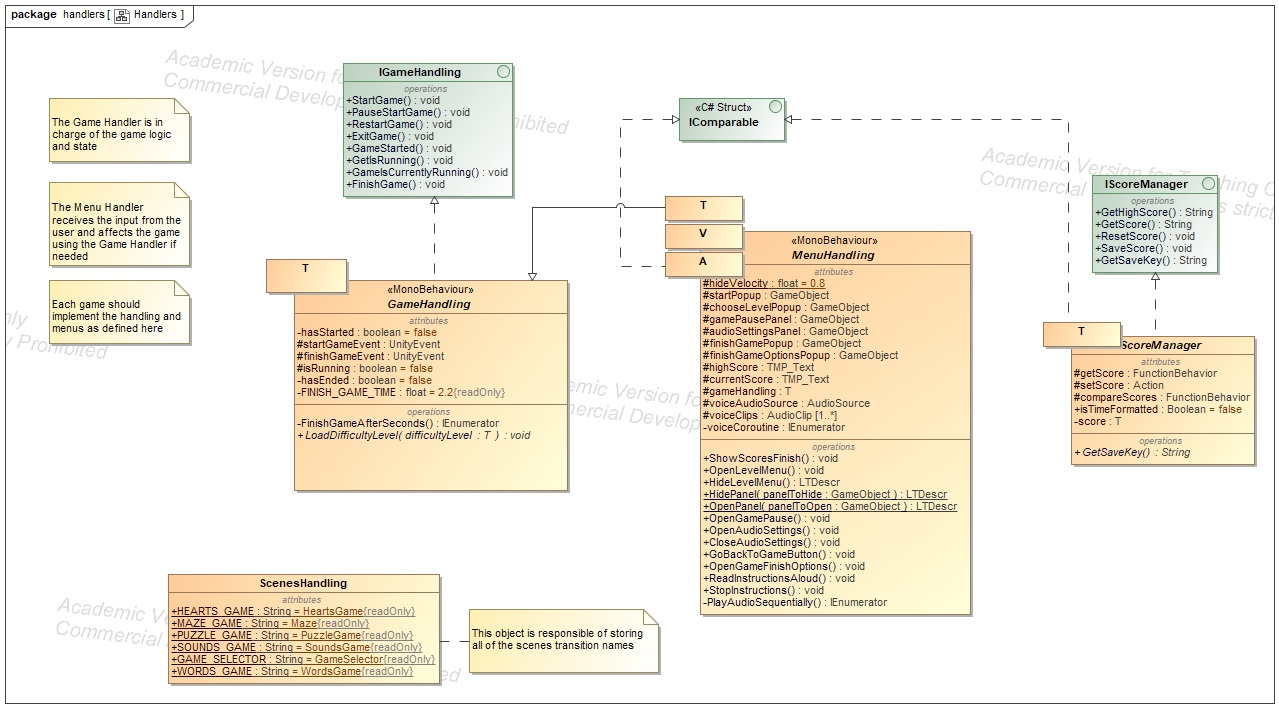
\includegraphics[width=\linewidth]{Chapters/new_architechture/class__handlers__Handlers.jpg}
    \caption{Handlers Mechanism \gls{uml}}
    \label{fig:handlers}
\end{figure}

\paragraph{Common}
% TODO: Finish and add the common diagram

The `Common' package hosts as the name implies all objects that although not being a part of the architecture can help simplify the process of development of the games. At this stage, only two classes were needed. 

The `Counter' behaviour will be used across multiple games. It is started through each GameHandling and, is able to communicate directly with the `ScoreManager'. This enables the counter to increase time through the `ScoreManager' object and update the correspondant \gls{ui}.

The `AudioSettings' behaviour handles the Audio Settings user interactions. It has access to all the Sliders in the Audio Menu (a slider is an existing Unity GameObject), each one is matched with a different mixer group. In Unity audio is handled with Mixers. The way the games were set up, each one has a mixer. Inside each mixer we can define multiple groups. Multiple groups were created for each game depending on the audio played, such as `Voice', `Background Music', `Notifications'. This allows each group to be controlled separately and also has the ability of adding audio filters for each one (such as low or high pass filters).

`ButtonAnimation' is a behaviour that is used in all of the games that set an expand and collide animation for the buttons in the game. Just like the rest of the \gls{ui} does, it utilizes the `LeanTween' external library for best results.

The `SetScaleZero' is an object that helps the developer work on any \gls{ui} component without having to worry about leaving everything as it was before. This class sets visible only the game start \gls{ui} components, keeping all others hidden.

Figure \ref{fig:common-classes} depicts the common package in \gls{uml}.
\begin{figure}[H]
    \centering
    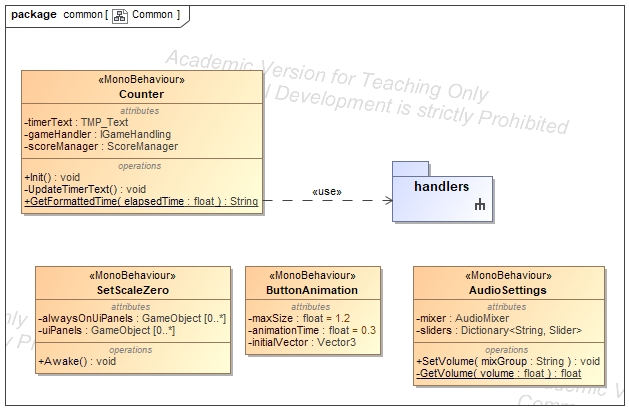
\includegraphics[width=0.8\linewidth]{Chapters/new_architechture/class__common__Common.jpg}
    \caption{Common Package \gls{uml}}
    \label{fig:common-classes}
\end{figure}

\section{Game 1 - Hearts}
\label{arqHearts}

The first game to be developed is the Hearts game, designed for young children between the age of 6 to 10 years old.

A significant entity in this game is the heart object that, as previously stated, may have different types and each one has a different impact on the scoreboard. For that, the ScriptableObject interface \cite{unityDocScriptableObj} comes in handy. This gives us the possibility of parametrizing each Heart to a  as well as a lifespan of that type of heart along with the score.

Another important aspect to tackle is the game settings. What this means is to parametrize the game into different difficulties so that the player can advance through each level as they learn along.
For this, we will also be using the ScriptableObject interface, taking into account the following aspects:

\begin{itemize}[noitemsep, topsep=5pt, parsep=5pt, partopsep=5pt]
    \item Spawn rate of the hearts on the screen.
    \item Type of heart to be spawned followed by the probability of that heart to be spawned.
    \item Time of the challenge.
\end{itemize}

These objects allow us to directly create a heart in the Unity Editor and attach the different characteristics we want for it. The same goes for the Game Settings, which makes it easier to change the level of the game or even add another one.

Every heart to be instantiated in the game has a behaviour. In this case, it has to affect the state of the game score and be immediately destroyed afterwards. This is handled through the `HeartScript' that is composed of a \textbf{Heart}.

To update the score, there is an implementation of the \textbf{ScoreManager}, the (`HeartScoreManager') that keeps track of the score as an integer.

Another problem to tackle is the random spawning of hearts. Any object to be instantiated will be a GameObject and therefore there needs to be a script to handle this behaviour. `HeartSpawner' is in charge of this, making sure to use the GameSettings to spawn each heart on the screen at different speeds and types of hearts.

Lastly, there is the `Bar' class used for handling the behaviour of the timer that advances according to the time boundaries of the game. This is done using \textit{LeanTween}, an extension of the Unity library that can be used to animate assets.

The following \gls{uml} diagram (Figure \ref{fig:heartsGameArq}) describes the Hearts game architecture.

\begin{figure}[H]
    \centering
    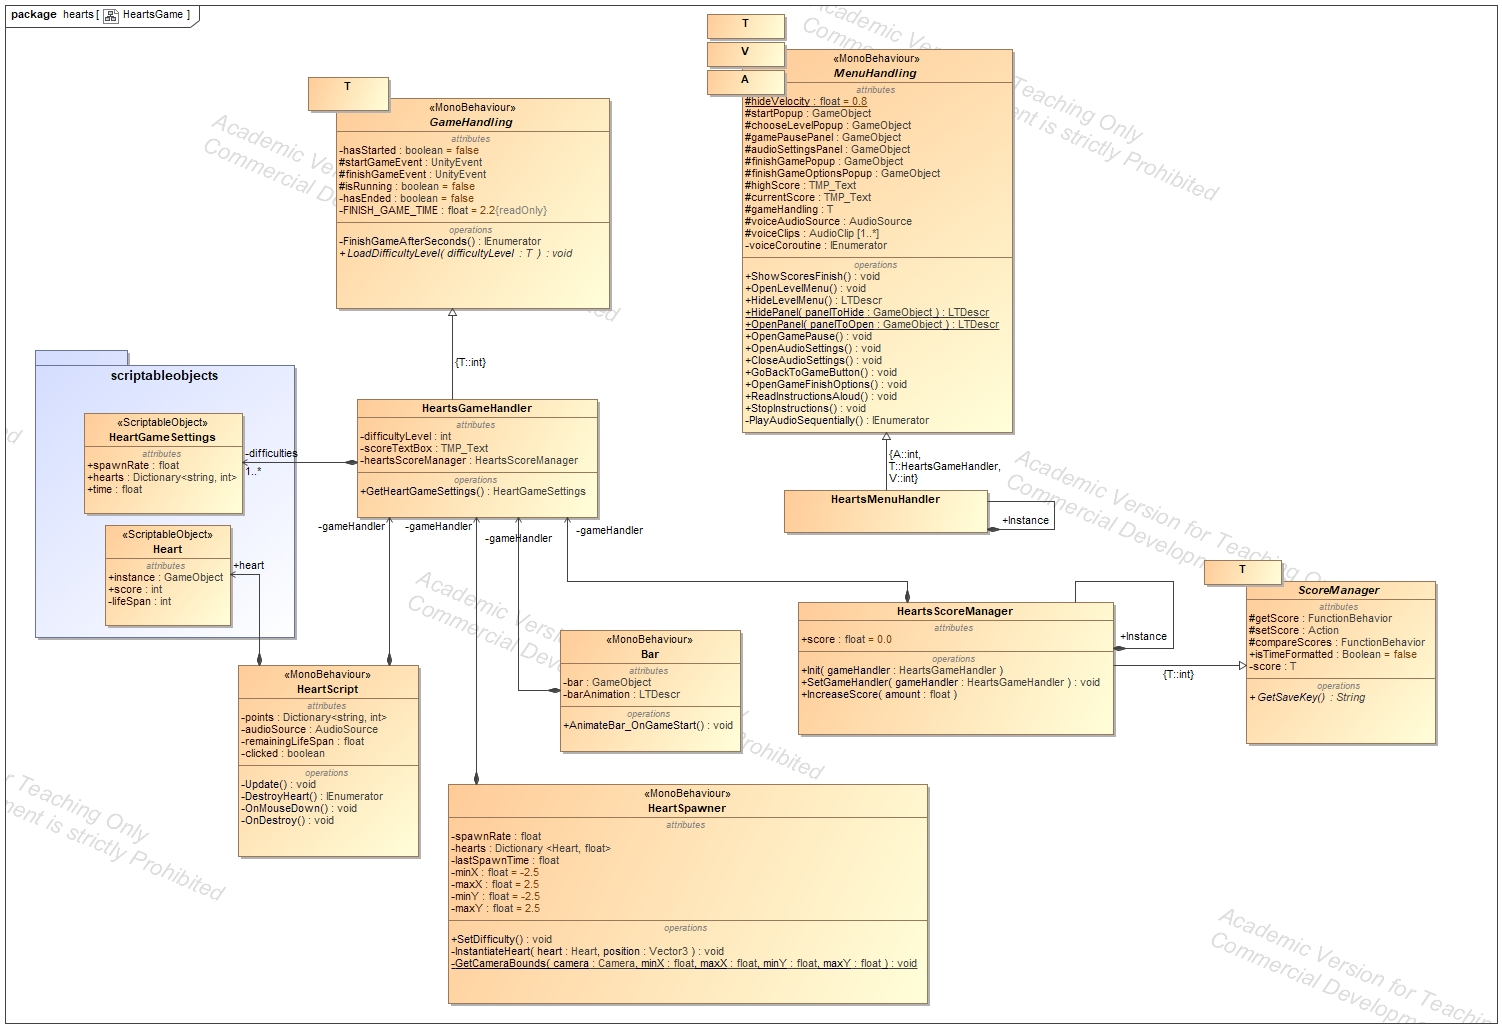
\includegraphics[width=\linewidth]{Chapters/new_architechture/class__hearts__HeartsGame.jpg}
    \caption{Hearts Game entities - \gls{uml}}
    \label{fig:heartsGameArq}
\end{figure}

\section{Game 2 - Maze}
\label{arqMaze}

The following \gls{uml} of Figure \ref{fig:mazeGameArq} represents the Maze Game arquitecture.

\begin{figure}[H]
    \centering
    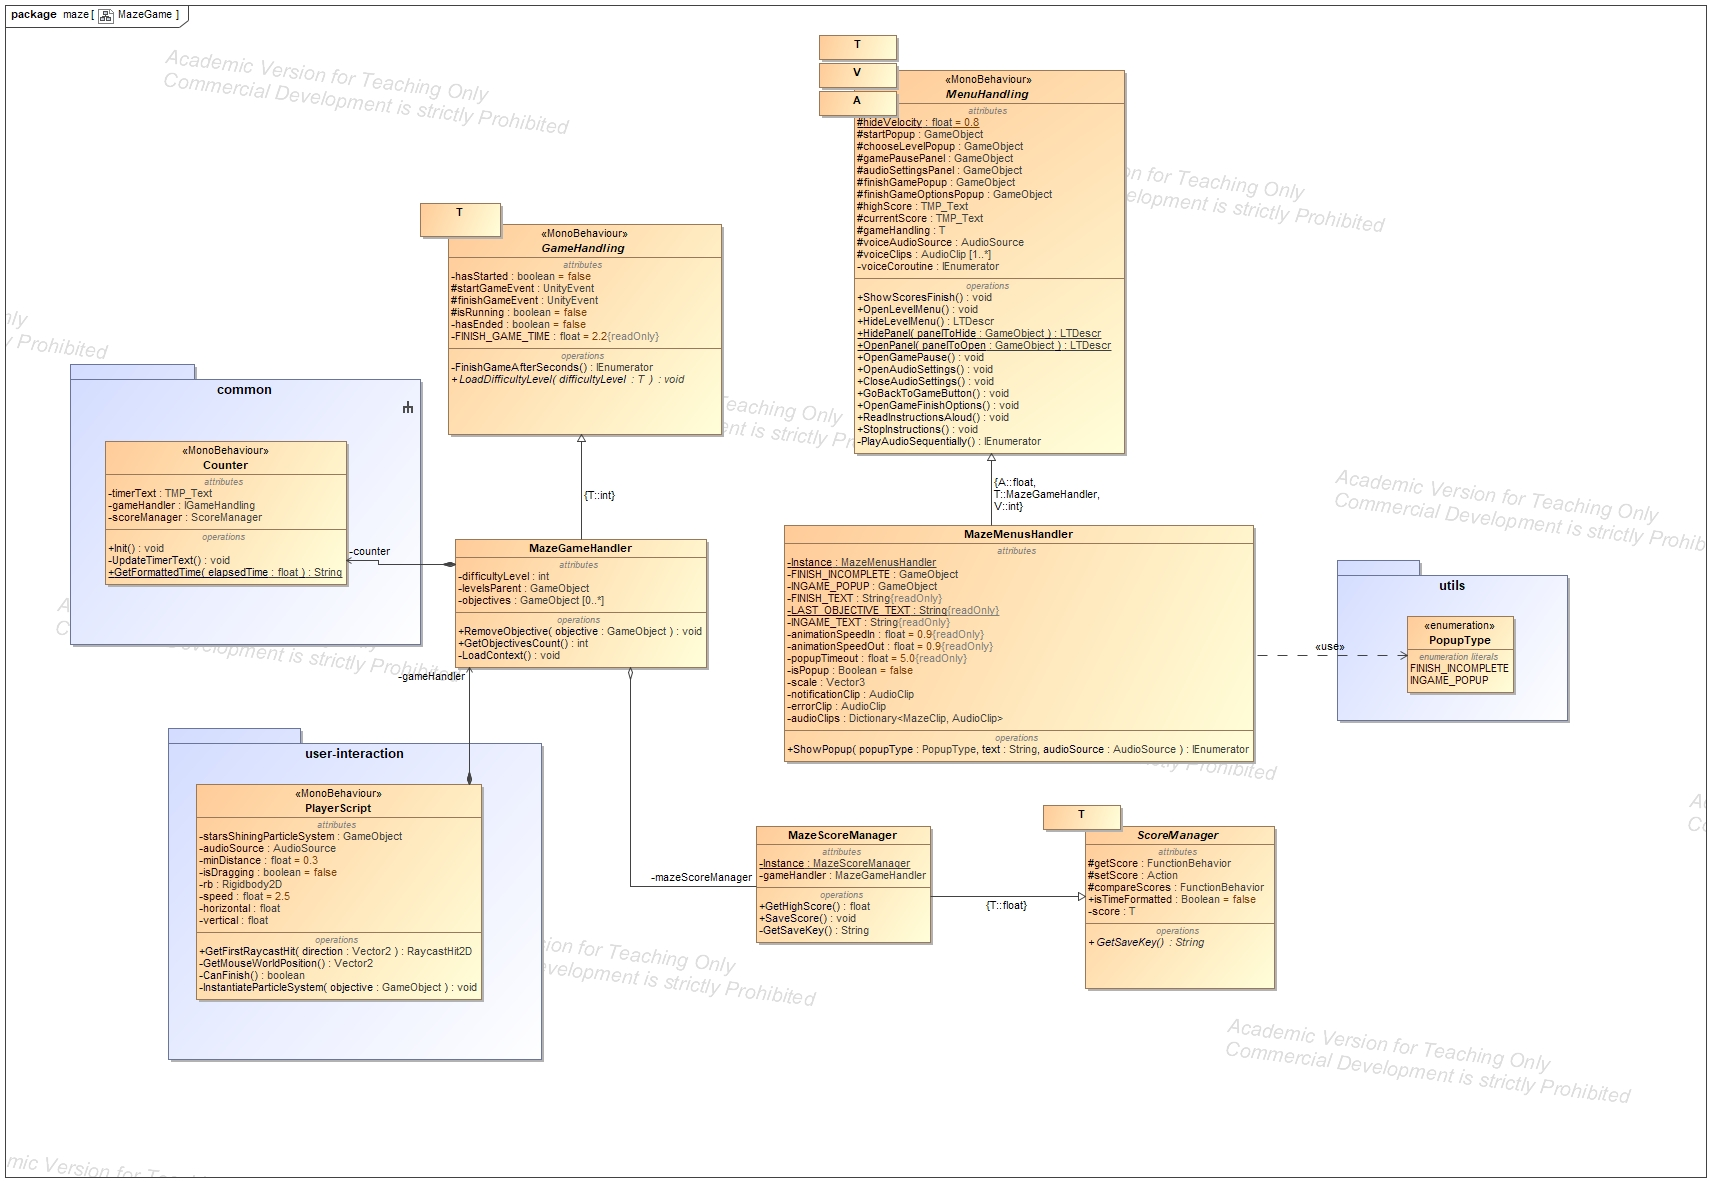
\includegraphics[width=\linewidth]{Chapters/new_architechture/class__maze__MazeGame.jpg}
    \caption{Maze Game Entities - \gls{uml}}
    \label{fig:mazeGameArq}
\end{figure}

The Maze Game consists of a map with a maze and multiple objectives the user has to attain before reaching the end of the maze. There are a couple of aspects to tackle.

The game has multiple levels, each one designed directly in Unity. The levels have inside the maze many objectives the player has to accomplish. For that, we utilized Unity's ability to tag GameObjects. Each objective has a tag and the player will play a certain logic given the tag of the catched object. All the objectives will be stored in a List structure and will be deleted as the player collects objectives.

The player movement is such that the user can have a choice of dragging the character through the path or using the Up, Down, Left, Right combination on the keyboard. All this logic is present in the `PlayerScript' behaviour located right at the player GameObject. The `PlayerScript' utilizes many `MonoBehaviour' methods such as `OnMouseDown', `OnMouseUp' and `OnTriggerEnter2D' to detect user drag and drop actions and player collision with objectives. It comunicates directly with the `GameHandling' to trigger finish events and update the game state.

There were also some popups implemented so that the user can get a notion of how the game is going. If the player tried to escape the maze before collecting all the objectives, this throws a popup reminding the player to go back, for example.

Lastly, the `Counter' was used to assess the time as score measurement and was directly wired to the implementation of `ScoreManager' (`MazeScoreManager').

\newpage
\section{Game 3 - Sounds}
\label{arqSounds}

The Sounds Game structure is as depicted in Figure \ref{fig:soundsGameArq}.

\begin{figure}[!h]
    \centering
    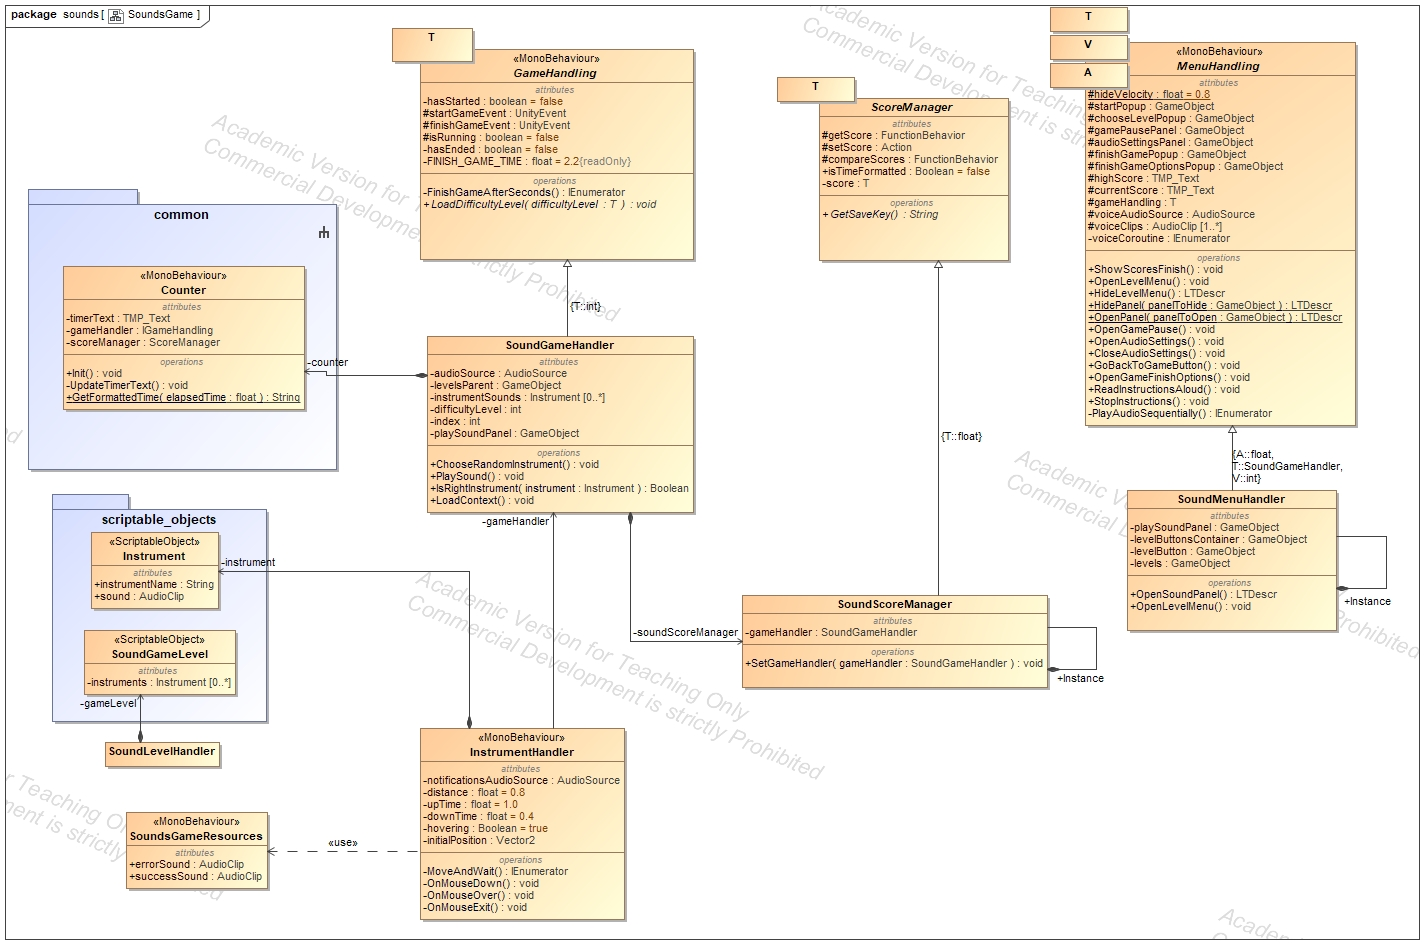
\includegraphics[width=\linewidth]{Chapters/new_architechture/class__sounds__SoundsGame.jpg}
    \caption{Sounds Game Entities - \gls{uml}}
    \label{fig:soundsGameArq}
\end{figure}

The Sounds Game's purpose is to let the player hear and find the instrument that is playing.

The are several levels in this game. Each one was created before hand, and consists of a map (background image) and multiple instruments scattered around this map. The player has a play button where one can play the instrument; after this, the game begins. The music starts and the player can hover over the instruments on the floor when once finds the correct one, one can click on it.

Each instrument on the floor was mapped to a \textit{ScriptableObject}, \textit{Instrument} which stores the instrument's name and its Sound, as an \textit{AudioClip} (\textit{Unity}'s implementation of audio objects). This Object is stored into the instrument's own handler, \textit{InstrumentHandler}, that utilize's \textit{Unity}'s mouse events to detect mouse clicks and hovering. This way, the handler can trigger \textit{LeanTween} animations. This object is also responsible of comunicating the \textit{SoundGameHandler} of which instrument is being clicked.

Each level was also mapped to a \textit{ScriptableObject}, \textit{SoundGameLevel} which hosts a list of all instruments available inside its level. All levels are present in the game scene inside a parent GameObject (all levels start disabled).

The \textit{SoundGameHandler} is the handler of this game and is able to load a certain level by accessing the parent object (\textit{levelsParent} attribute) and loading a certain level, gathering all its instruments to the attribute \textit{instrumentSounds}.
It has a method capable of validating if the right instrument is being clicked \textit{IsRightInstrument} (triggered by \textit{InstrumentHandler}).
This object also plays the instrument's sound for the player to listen.

This game's score metric is also the \textit{Counter} from previous games, being again instantiated by the game handler.

\section{Game 4 - Words}
\label{arqWords}

The Words Game architecture is depicted in Figure \ref{fig:wordsGameArq}.

\begin{figure}[!h]
    \centering
    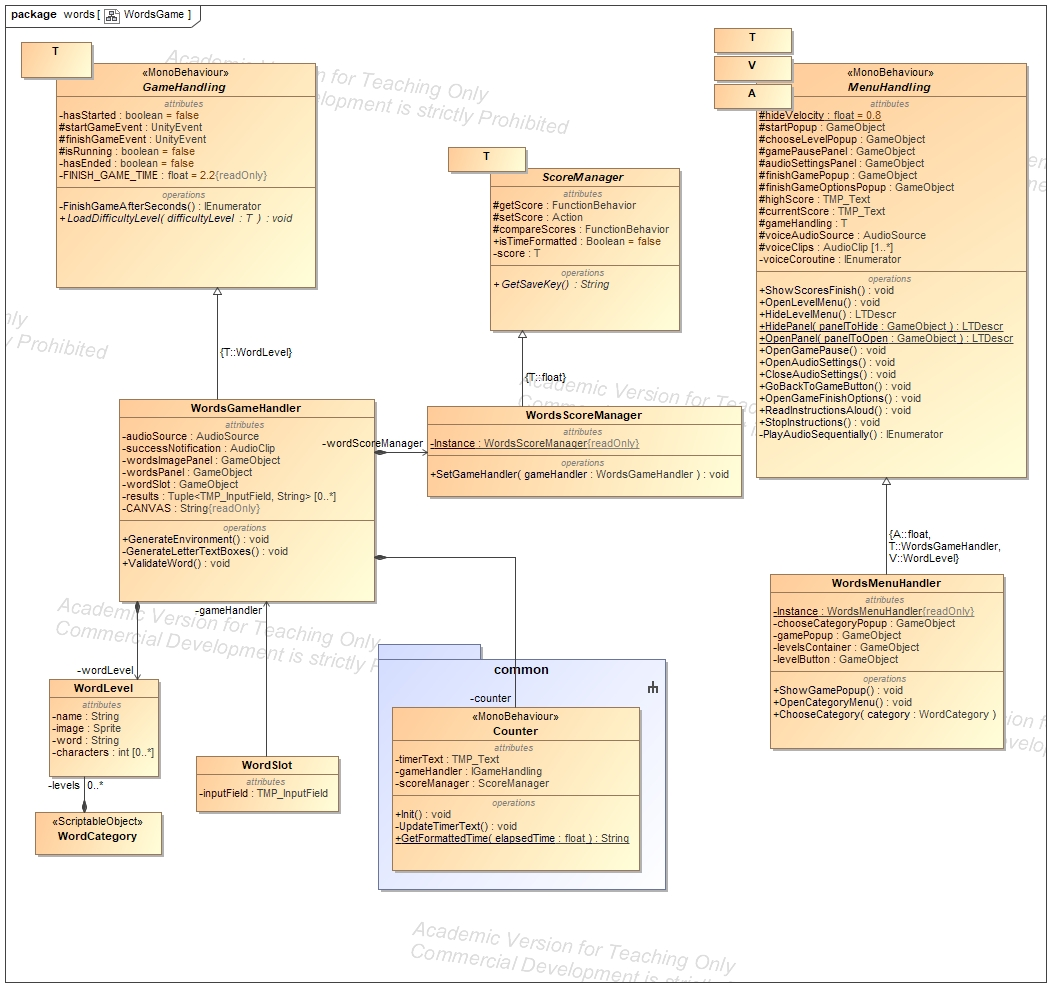
\includegraphics[width=\linewidth]{Chapters/new_architechture/class__words__WordsGame.jpg}
    \caption{Words Game Entities - \gls{uml}}
    \label{fig:wordsGameArq}
\end{figure}

This game's purpose is to find the word that describes the image being displayed. Like defined before, there are two categories for these images: \textit{Nature Objects} and \textit{Industrial Objects}.

Each game category was mapped to a \textit{ScriptableObject} which is composed of multiple levels inside. Each level is a \textit{Word Level} that is also a \textit{ScriptableObject}. Each \textit{WordLevel} has a name, an associated image, a complete word and a list of characters that define which characters are visible and which ones aren't.

The \textit{WordsGameHandler} is capable of generating an environment (\textit{GenerateEnvironment} method together with \textit{GenerateLetterTextBoxes}) from this \textit{WordLevel} alone. This environment is an \gls{ui} that has the current word's image and multiple text box slots where the player can type the word according to the image (some slots come pre-filled depending on the \textit{WordLevel} hiding \textit{characters}).

Each slot was also assigned to a \textit{WordSlot} object, that it's main responsability is to validate the word every time any Word Slot text changes. For this, it utilizes the \textit{WordsGameHandler}'s \textit{ValidateWord} method.

The GameHandler also uses the \textit{Counter} as a score metric, being stored as a float in the \textit{WordsScoreManager}.

\section{Game 5 - Puzzle}
\label{arqPuzzle}

The Puzzle Game was defined as depicted in Figure \ref{fig:puzzleGameArq}.

\begin{figure}[!h]
    \centering
    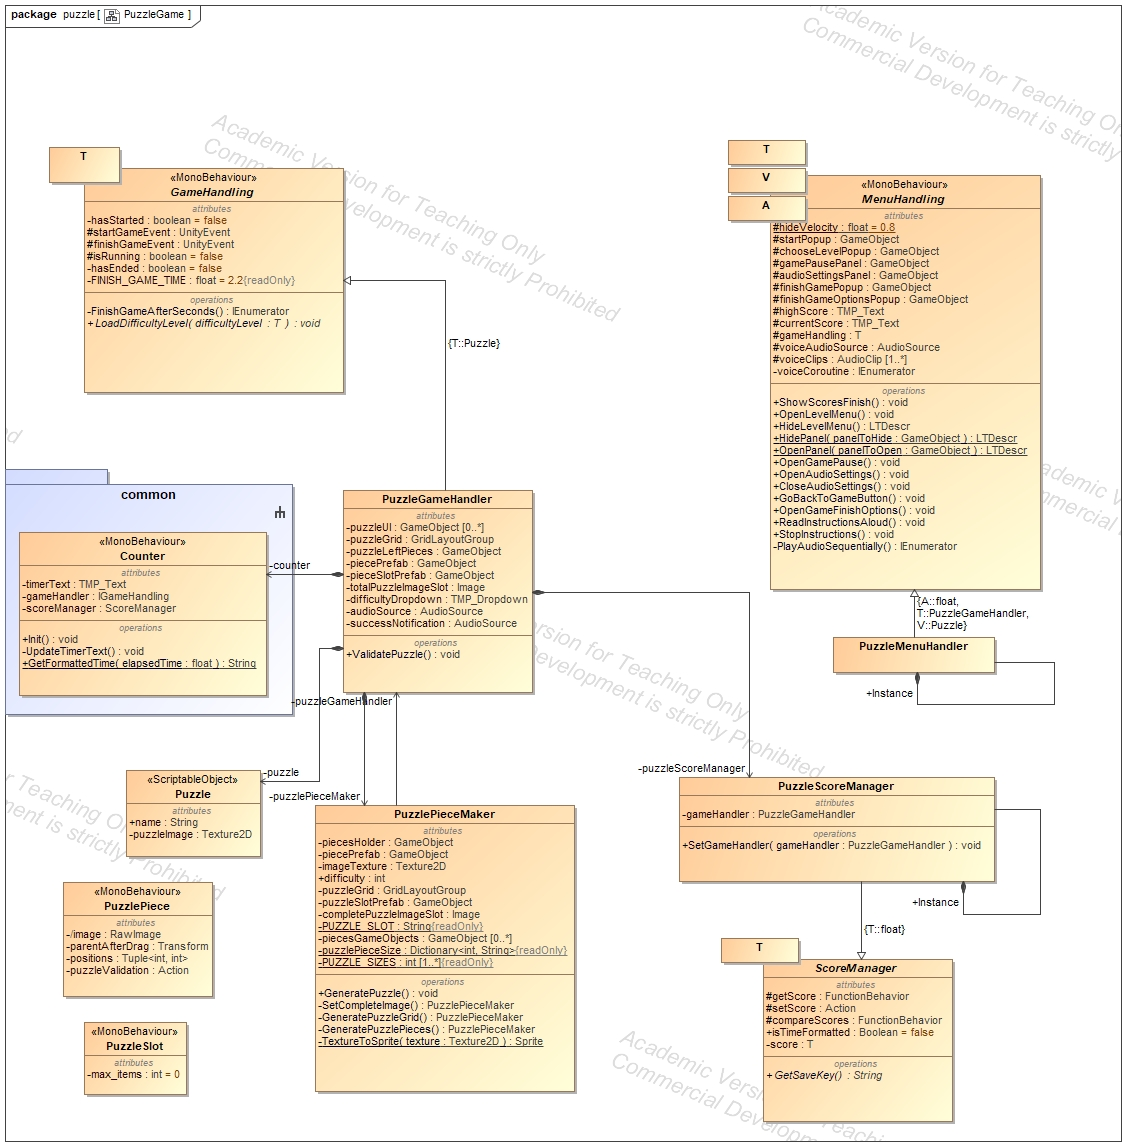
\includegraphics[width=\linewidth]{Chapters/new_architechture/class__puzzle__PuzzleGame.jpg}
    \caption{Puzzle Game Entities - \gls{uml}}
    \label{fig:puzzleGameArq}
\end{figure}

The purpose of the game is for the player to complete puzzles. The first aspect defined was how it would be played. After some thinking, the best way to do it would be with three main components on the screen:

\begin{itemize}
    \item Complete Puzzle Image.
    \item Puzzle Grid to place pieces.
    \item All puzzle pieces in a tray.
\end{itemize}

The grid and the tray both used Unity's \gls{ui} grid layout group, which is a component that organizes its children in a grid-like way. The puzzle grid would have multiple placeholders (each placeholder is a `PuzzleSlot') for the puzzle depending on the difficulty (3x3 or 5x5 grid for instance).

The player has to be able to drag and drop pieces from the tray to the placeholders on the puzzle grid. This mechanism utilizes Unity's methods `OnBeginDrag', `OnEndDrag', `OnDrag' from the IBeginDragHandler, IDragHandler, and IEndDragHandler interfaces.
% TODO: add puzzle piece interfaces realization
% TODO: add all unity event functions to 

For faster level creation it was also decided the game itself has to be able to cut any image into puzzle pieces. This way, we can introduce new levels to the game by simply adding an image.

All these functionalities are present in the `PuzzlePieceMaker' class with the following methods:

\begin{itemize}
    \item SetCompleteImage.
    \item GeneratePuzzleGrid.
    \item GeneratePuzzlePieces.
\end{itemize}

This object is used in the game handler (`PuzzleGameHandling') and uses the `Puzzle' object, a `ScriptableObject' that holds each puzzles name and texture image.

Like some other games, this one also uses the `Counter' mechanism as a way to store scores in its `PuzzleScoreManager'.

% DONE: PRF No capitulo 4, e importante discutir e apresentar os seguintes topicos:
% As razoes de escolha do paradigma OOP
% - do C#
% - do Unity
% quais criterios seguidos em termos de resolucao das imagens, cores, etc., ou seja, todos os aspetos de interface do utilizador